%% -*- coding: utf-8 -*-
\documentclass[12pt,pagesize,paper=192mm:108mm]{scrbook} 
%1920x1080 1280x720
\areaset[current]{192mm}{108mm}
\usepackage{calc}
\usepackage[T2A]{fontenc}
\usepackage[utf8]{inputenc}
\usepackage[english,russian]{babel}
\usepackage{microtype}
\usepackage{misccorr}
\usepackage{cmap}
%\usepackage[unicode=true]{hyperref}
\usepackage{graphicx}
\usepackage{amssymb}
\usepackage{amsmath}
%\usepackage{srcltx}
\usepackage{textcomp}
\usepackage{xspace}
%научные символы и смайлики \smiley \frownie
\usepackage{wasysym}
\usepackage{ccicons}
\begin{document}
\begin{titlepage}
  \vspace*{-0.5em}
  \begin{center}    
    \hspace*{3em}
    \begin{minipage}[t]{3em}
      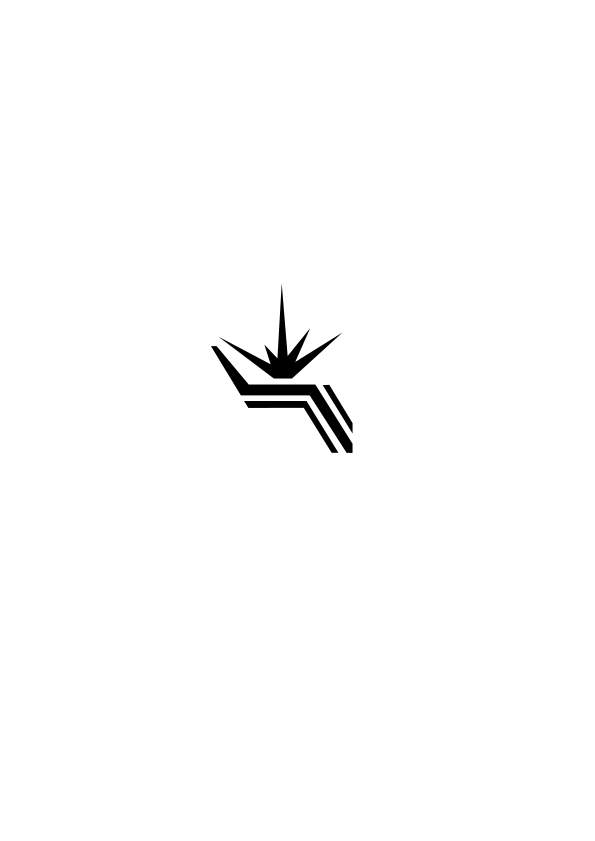
\includegraphics[width=\textwidth]{../BINP-logo}
    \end{minipage}\hfill
    \begin{minipage}{0.23\linewidth}
    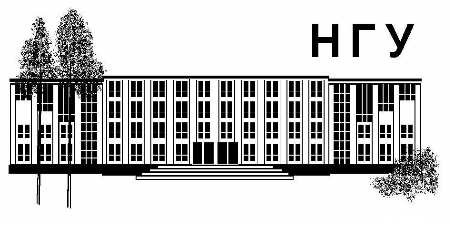
\includegraphics[width=\textwidth]{../NSU-logo}
    \end{minipage}
    \hfill
    \hspace*{6em}

    Кафедра теоретической физики физического факультета НГУ
    \medskip

    \Large
    Профессор Фадин В.\,С.
    \bigskip

    \huge
    \textbf{Квантовая электродинамика}
    \bigskip

    \Large
    Лекция № 5
    \vfill

    \normalsize
    % \begin{minipage}{0.65\linewidth}
    % \end{minipage}
    \vfill

    \normalsize \ccbysa\hspace{0.5em}  Новосибирск 2013
  \end{center}
\end{titlepage}
\vspace*{-1em}
\begin{center}
\vfill
  \begin{minipage}{0.85\linewidth}
    Процессы электрон"=пионного рассеяния $e \pi \to e \pi$ и
    аннигиляции $e^+e^-\to\pi^+\pi^-$ и измерение формфактора
    $\pi$-мезона. Формфактор $\pi$-мезона в канале аннигиляции вблизи
    $\rho$-мезона. Полное сечение вблизи векторного резонанса.
    Рассеяние электрона на протоне: вершина взаимодействия фотона с
    протоном, формфакторы протона. Сечение рассеяния электрона на
    протоне в борновском приближении (формула
    Розенблюта). Электрический и магнитный формфакторы
    протона. Поведение формфакторов с ростом передачи импульса,
    поведение отношения формфакторов. Поляризационные эксперименты
    по~измерению отношения формфакторов. Противоречие между данными,
    полученными в~поляризационных экспериментов и методом
    розенблютовского разделения.  Диаграммы двухфотонного
    обмена. Разность сечений рассеяния электронов и позитронов
    на~протоне. Кросс-канал аннигиляции $e^+e^- \to p\bar{b}$,
    пороговое поведению сечений, роль кулоновского взаимодействия
    конечных частиц, связанные состояния ниже порога реакции,
    дифференциальное сечение. Сингулярности амплитуд и соотношение
    унитарности.  Дифференциальное сечение реакций $e\mu \to e\mu$ и
    $e^+e^- \to \mu^+\mu^-$, зависимость сечения аннигиляции от
    скорости мюонов, угловое распределение, полное сечение, сравнение
    с $e^+e^- \to \pi^+\pi^-$, кулоновское взаимодействие частиц в
    конечном состоянии, фактор Зоммерфельда"--~Сахарова.
  \end{minipage}
  \vfill

  % \normalsize \ccbysa\hspace{0.5em} Новосибирск 2013
\end{center}
\end{document}
